

\chapter{Conclusion}

At the beginning of the LHC physica program, there was much hope for the
resolution of a number of open issues in particle physics and the potential
discovery of a plethora of new particles.
In some ways, the first years of the LHC was an immense success.
The high energies and luminosities coupled with the incredibly powerful
and precise particle detectors led to measurements with incredible
accuracy.

\begin{figure}[ht!]
  \begin{center}
    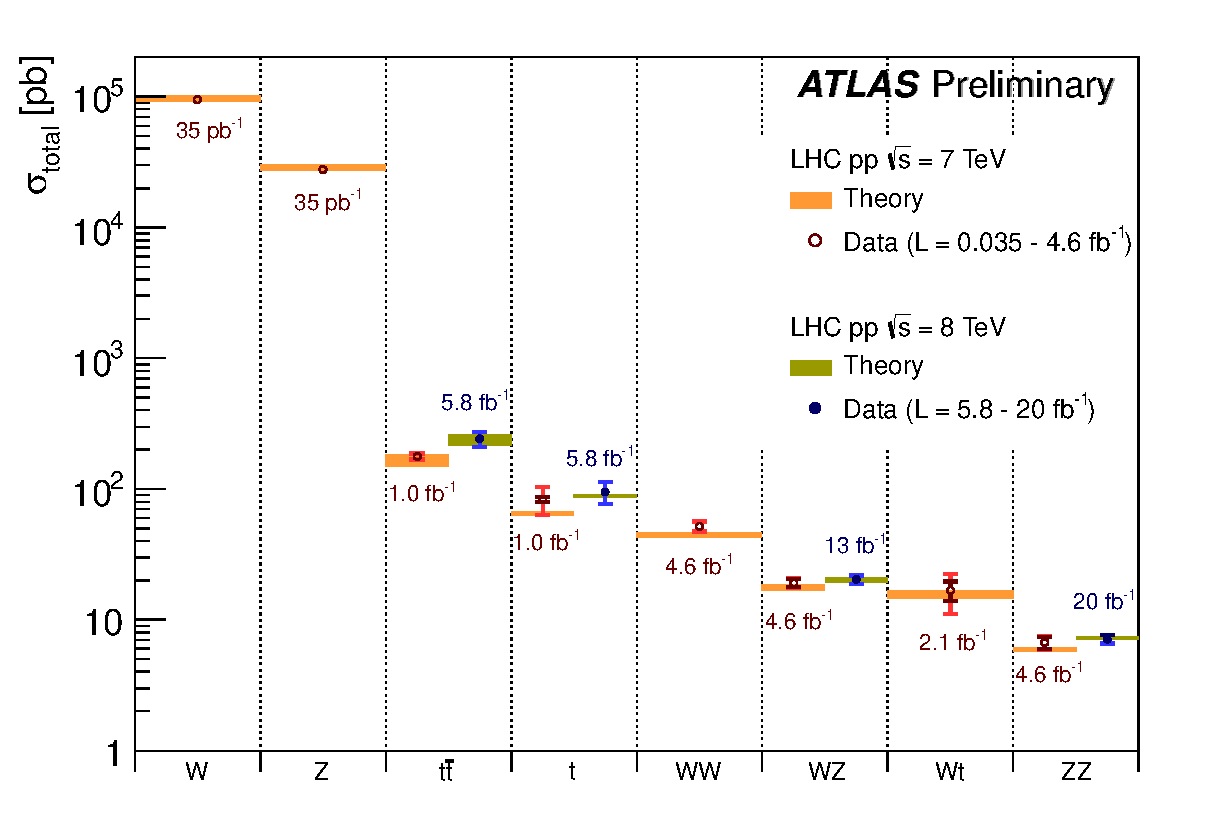
\includegraphics[width=.75\textwidth]{figures/conclusion/SM_SummaryPlotMoriondEWK2013}
    \caption{Things}
    \label{fig:xsec_vs_roots}
  \end{center}
\end{figure}


Among these are many detailed studies of the top quark, which levered
advanced experimental and statistical techniques to achieve world class measurements.
This thesis described a number of analyses which resulted in world class measurments
of the top quark pair-production cross-section, including a statistical combination
of analyses that resulted in the most powerful measurement of the $\ttbar$ cross
section measured at the LHC at the time.

\begin{figure}[ht!]
  \begin{center}
    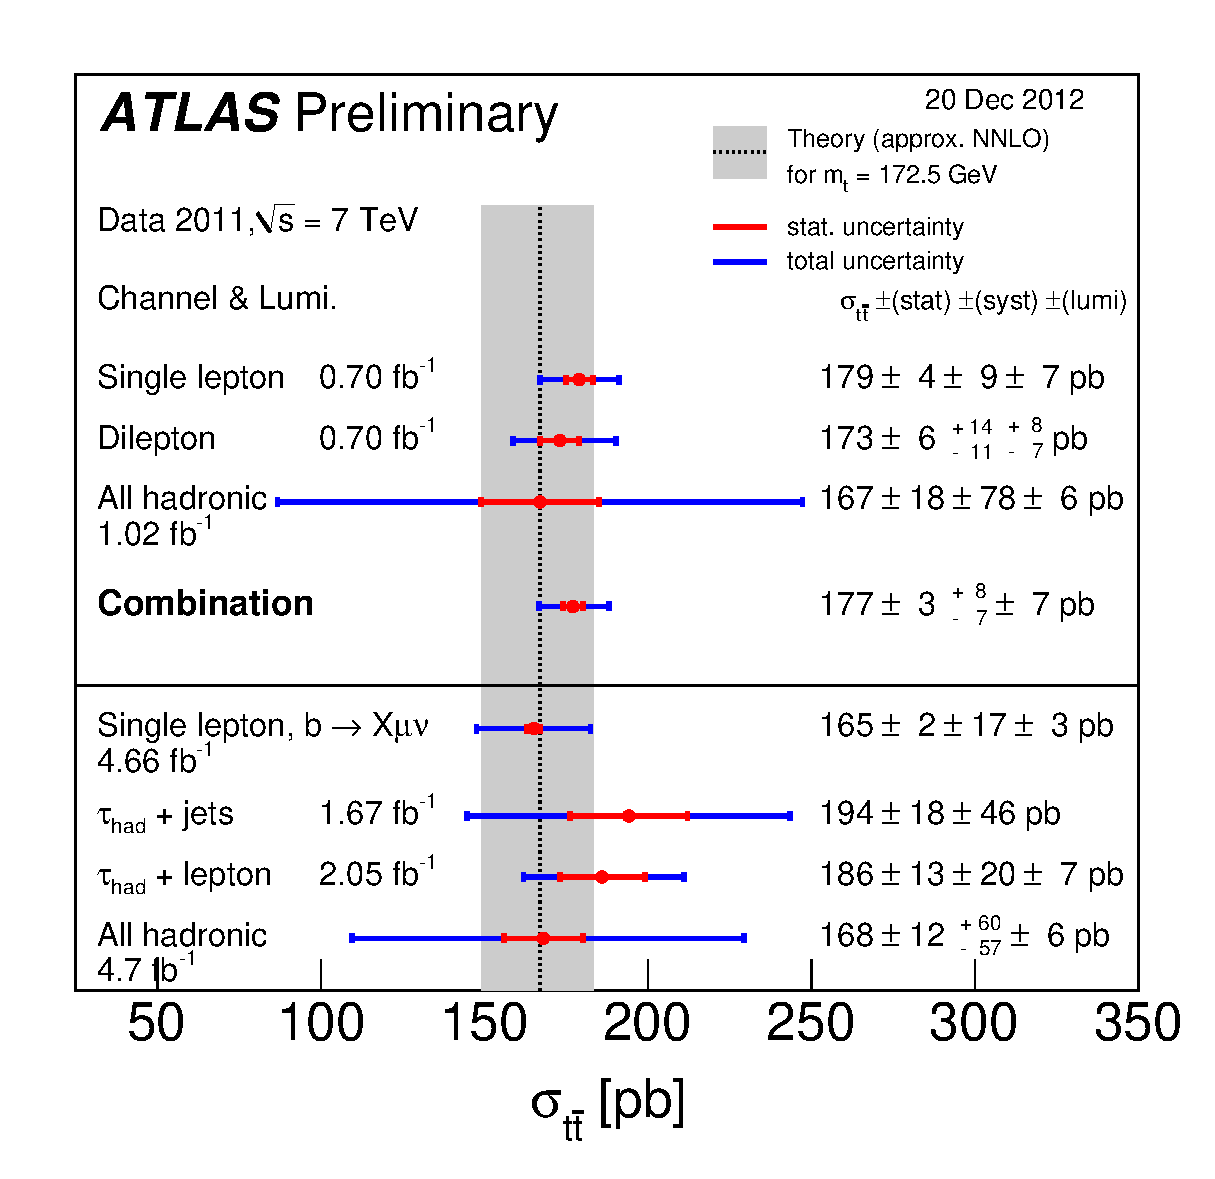
\includegraphics[width=.75\textwidth]{figures/conclusion/tt_xsec20Dec2012}
    \caption{Things}
    \label{fig:xsec_vs_roots}
  \end{center}
\end{figure}
\clearpage

Cheif among the successes of the early LHC program was the discovery of the Higgs boson.
However, motived by the hierarchy problem, many had hoped that the mechanism of electroweak
symmetry breaking would be more rich than the Higgs mechanism of the Standard Model and
would bring with it a number of new particles.
Many had hoped that the discovery of SuperSymmetry would lead to a more natural understanding
of electroweak symmetry breaking.
However, extensive studies on numerous supersymmetric models have yet to find evidence
supporting the existance of supersymmetric partners.

\begin{figure}[ht!]
  \begin{center}
    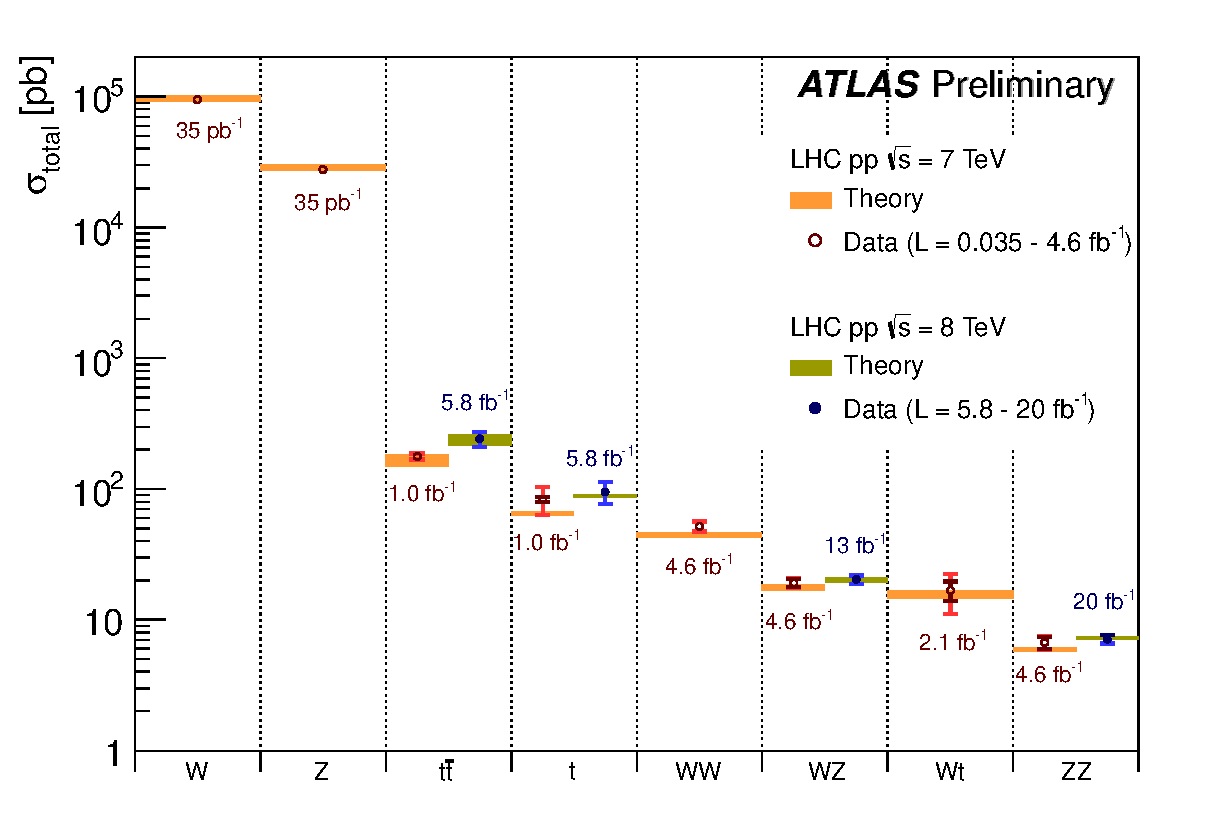
\includegraphics[width=.75\textwidth]{figures/conclusion/SM_SummaryPlotMoriondEWK2013}
    \caption{Things}
    \label{fig:xsec_vs_roots}
  \end{center}
\end{figure}
\clearpage

In addition to spectrum of Supersymmetric models, the experiments at the LHC have searched
for more exotic physical models, many of which were theorized to address the hierarchy
problem and other shortcomings of the Standard Model.

\begin{figure}[ht!]
  \begin{center}
    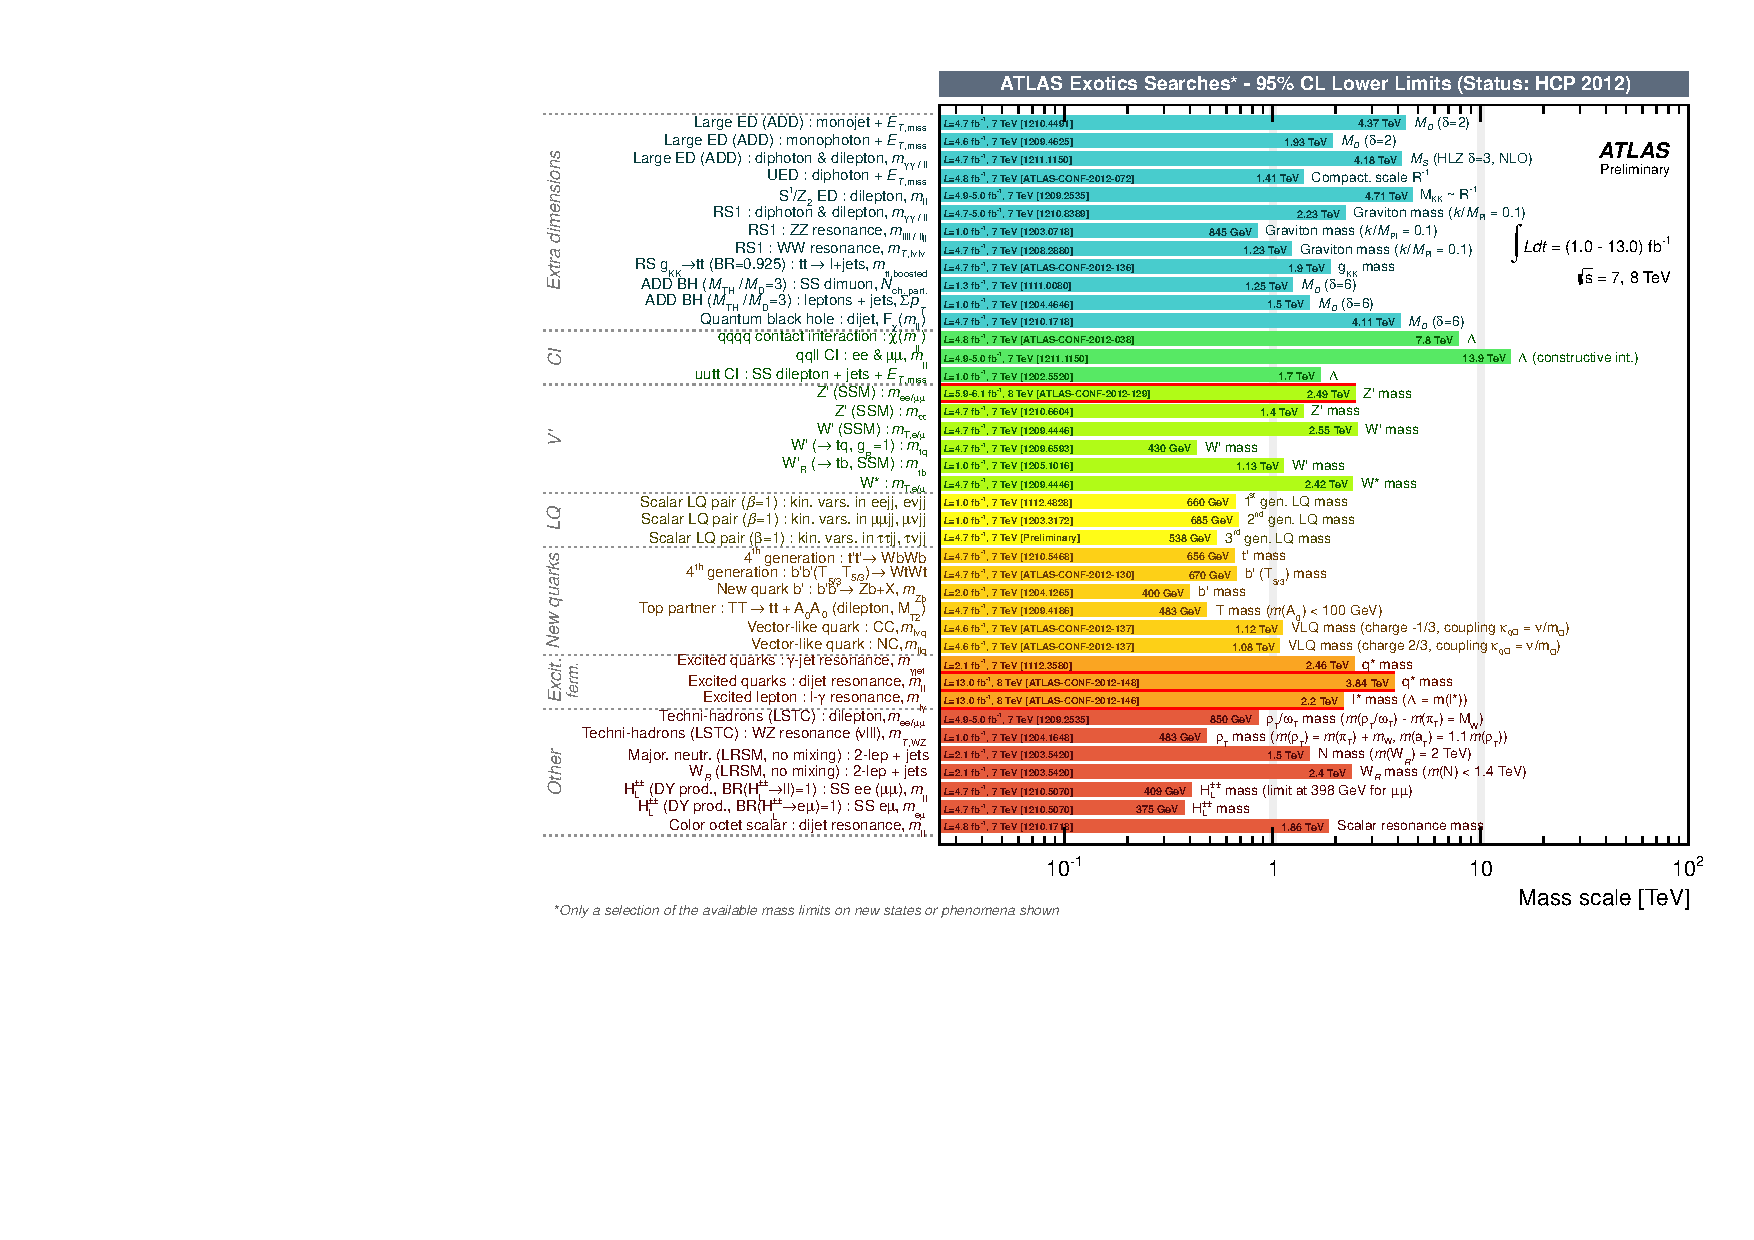
\includegraphics[width=.75\textwidth]{figures/conclusion/ExoticResultsSummary}
    \caption{Things}
    \label{fig:xsec_vs_roots}
  \end{center}
\end{figure}

This thesis described a search for exotic processes in the same-sign dilepton plus jets signature that
was aimed at discovering a number of potential particles, including particles from models that provide
exotic explanations of the hierarchy problem.
However, no evidence supporting these models was found in the data.
